%% Engineering Applications of Artificial Intelligence (Elsevier) -- elsarticle, review layout.
%% Compile on Overleaf (pdfLaTeX + BibTeX). Tables in tables/ are generated by scripts/49_paper_latex.py:
%% do not edit them by hand. Every claim must be in claims.md.
\documentclass[review,12pt]{elsarticle}

\usepackage{amsmath,amssymb}
\usepackage{booktabs}
\usepackage{graphicx}
\usepackage{xcolor}
\usepackage{tikz}
\usetikzlibrary{arrows.meta,positioning,shapes.geometric}
\usepackage[hidelinks]{hyperref}
\usepackage{lineno}
\linenumbers

% Numbers that depend on the pending Qwen2.5-7B first-proposal-only run are wrapped in \pending{}.
\newcommand{\pending}[1]{\textcolor{red}{#1}}
\newcommand{\todo}[1]{\textcolor{orange}{[TODO: #1]}}

\journal{Engineering Applications of Artificial Intelligence}

\begin{document}

\begin{frontmatter}

\title{Knowing when to skip the simulator: model-internal signals for selective validation of LLM agent actions in process control}

\author[ic]{Javal Vyas\corref{cor1}}
\ead{j.vyas24@imperial.ac.uk}
\author[ic]{\todo{co-authors}}
\cortext[cor1]{Corresponding author}
\address[ic]{\todo{Department}, Imperial College London, London, United Kingdom}

\begin{abstract}
Large language model (LLM) agents that propose recovery actions for industrial processes are usually guarded by a
digital-twin validator that checks every proposal before execution. Validation cost grows with simulation fidelity and
horizon, whereas the agent's own forward pass costs a fixed amount. We ask when the validator can be skipped safely,
and which signals tell us so: observable features of the task and proposed action, or the model's token confidence,
attention, hidden states and a region-based attention grounding signal that measures whether the model attended to the
part of the prompt that decides its answer. In a pre-registered study with sealed test sets, five open-weight models
and two domains (graph path planning with an exact validator, and fault recovery for a continuous stirred-tank
reactor), learned risk screens skipped 16--91\% of validator calls, with certified failure bounds where the accepted
set was large enough. Internal signals added 5--15 points of skipped calls for four of five models in path planning,
where failures stem from not consulting the relevant information, but helped only one to three models in the reactor
task, where models attend to the relevant physics and reason incorrectly. In 400 fresh closed-loop episodes per
model, probes using internal signals accepted failing retries for two models; allowing unchecked execution only for
first proposals removed this failure while keeping recovery. Because screening cost is independent of simulation
fidelity, savings grow with validator cost, reaching \pending{21--64\%} of total compute at 60\,s per validation for
four of five models.
\end{abstract}

\begin{keyword}
Large language models \sep Selective verification \sep Digital twin \sep Fault-tolerant control \sep
Model internals \sep Risk certification
\end{keyword}

\end{frontmatter}

\section{Introduction}\label{sec:intro}

Large language model (LLM) agents are increasingly used to propose supervisory actions for engineered systems:
recovery setpoints after a process fault, operating sequences, or plans that a lower-level controller then executes
\citep{yao2023react,shinn2023reflexion,car_todo}. Because an LLM's proposal can be wrong in ways that are hard to
anticipate, such agents are usually deployed behind a \emph{validator}: every proposal is checked by a simulator or
digital twin before it reaches the plant, and rejected proposals are returned to the agent with feedback. This
propose--validate--retry loop makes the agent safe by construction, but it makes every decision pay for a full
validation. Validation is often the expensive step: a digital-twin rollout must simulate the plant over the recovery
horizon, and its cost grows with the horizon, the model fidelity and the number of scenarios checked, while the cost
of the agent's own forward pass is fixed for a given prompt.

This raises a practical question: \emph{when can the validator be skipped, and how do we know?} A screen that
predicts, before validation, whether a proposal will pass could execute confident proposals directly, send clearly
bad proposals straight back to the agent, and validate only the uncertain ones. For such a screen to be useful in an
engineering setting, three things must hold. Its accept decisions must come with a guarantee on the failure rate of
what is executed unchecked; its decisions must remain safe when used inside the closed loop, not only on a static test
set; and its own cost must be small relative to the validation it replaces.

Two families of signals are available to such a screen. \emph{Observable} features describe the task state and the
proposed action, for example the plant measurements and the size of the proposed setpoint change; they are cheap but
domain specific. \emph{Model-internal} signals come from the agent itself: the confidence of its output tokens
\citep{kadavath2022know}, its hidden states \citep{azaria2023internal,burns2023ccs}, and its attention. Internal
signals are attractive because they are available for any task without a model of the plant, and because attention
offers a mechanistic reading: if the model did not attend to the part of the prompt that decides the answer, its answer
is suspect, a principle recently exploited for detecting contextual hallucinations \citep{chuang2024lookback}. We
call this signal \emph{region-based attention grounding}.

This paper studies, in a pre-registered and certification-oriented design, how many validator calls each signal lets
an LLM agent skip, at what risk, and at what cost. We use two domains with a validator in the loop: a graph
path-planning task in which every proposal is checked exactly, and fault recovery for a continuous stirred-tank
reactor (CSTR) in which proposals are validated by a digital twin \citep{car_todo}. Five open-weight models from three
families (Qwen2.5 1.5B, 3B and 7B \citep{qwen2025}, Llama-3.2-3B \citep{llama3} and SmolLM2-1.7B
\citep{allal2025smollm2}) generate the proposals.

Our contributions are as follows.
\begin{enumerate}
\item \textbf{A skip-the-validator protocol with certified accepts.} Each proposal is accepted unchecked, rejected
unchecked, or validated, using thresholds frozen on development data and a one-sided Clopper--Pearson bound on the
failure rate among unchecked accepts (Section~\ref{sec:method}). All hypotheses, rules and amendments were
pre-registered, and every test partition was evaluated once.
\item \textbf{A comparison of signals across two domains and five models.} Learned screens skip 16--91\% of validator
calls. Model internals add 5--15 points for four of five models in path planning, but only for one to three models,
each in a different way, in CSTR fault recovery (Section~\ref{sec:results}).
\item \textbf{A mechanistic account of when internals help.} Low attention on the deciding prompt region predicts
failure strongly in path planning (AUROC 0.75--0.88), where errors come from not consulting the relevant information,
and weakly or not at all in CSTR (0.48--0.72), where the model attends to the relevant physics and reasons
incorrectly.
\item \textbf{Closed-loop evidence and a deployment rule.} On 400 fresh CSTR episodes per model, trained screens
executed far fewer failing actions than random skipping at matched rates. Probes that use internal signals failed on
retries, whose prompts contain failure feedback, for two models; allowing unchecked execution only for first
proposals removed these failures with no measurable loss of recovery (Section~\ref{sec:closedloop}).
\item \textbf{A cost analysis that ties savings to simulator fidelity.} Because decisions do not depend on validator
latency, the logged closed-loop decisions can be re-costed exactly. Savings are small or negative for a fast
validator and grow to 21--64\% of total compute at 60\,s per validation for four of five models; we report the
break-even validator cost for every screen.
\end{enumerate}

The remainder of the paper reviews related work (Section~\ref{sec:related}), defines the screens, signals and
certification procedure (Section~\ref{sec:method}), describes the domains and data (Section~\ref{sec:setup}), and
reports offline results (Section~\ref{sec:results}), closed-loop results and costs (Section~\ref{sec:closedloop}).
Section~\ref{sec:discussion} discusses implications and limitations.

\section{Related work}\label{sec:related}

\paragraph{LLM agents with validators} Agent frameworks interleave reasoning with actions and use environment
feedback to revise proposals \citep{yao2023react,shinn2023reflexion}. In process systems, LLM agents have been used
for supervisory fault recovery, where proposals are checked against plant knowledge and digital-twin rollouts before
execution \citep{car_todo}. These designs treat validation as mandatory; we ask when it can be skipped and quantify
the safety and compute consequences. \todo{add 2--3 references on LLMs for process control and fault-tolerant control.}

\paragraph{Selective prediction and risk control} Selective classification lets a model abstain when its risk is
high, trading coverage for accuracy \citep{geifman2017selective}. Distribution-free methods calibrate such decisions
to guarantee a risk level with high probability \citep{bates2021rcps,angelopoulos2021ltt}. Our accept rule follows
this tradition: thresholds are chosen on development data so that an upper confidence bound on the failure rate of
accepted proposals stays below a tolerance, and the guarantee is checked once on an independent certification set
with an exact binomial bound \citep{clopper1934}. Unlike standard selective prediction, the screen has three outcomes
(accept, reject, validate) and the cost of a reject is a regeneration by the agent, which we measure in closed loop.

\paragraph{Uncertainty and internal states of LLMs} LLMs' token probabilities carry information about answer
correctness \citep{kadavath2022know}, and linear probes on hidden states detect falsehoods and latent knowledge
\citep{azaria2023internal,burns2023ccs}. Semantic entropy detects confabulations from sampled answers
\citep{farquhar2024semantic}, and probes can approximate it from a single forward pass \citep{kossen2024sep}. These
works ask whether an answer is likely wrong; we ask how many validator calls such signals let an agent skip at a
certified risk, compare them with strong observable baselines, and test them in closed loop.

\paragraph{Attention as evidence of grounding} Whether attention weights explain model behaviour is debated
\citep{jain2019attention,wiegreffe2019attention}; we use attention only as a predictive signal. Lookback Lens
detects contextual hallucinations from the ratio of attention on the context to attention on generated tokens
\citep{chuang2024lookback}. Our region-based grounding is closer to a targeted version of this idea: it measures the
share of attention, while writing each decision-relevant token, that falls on the specific prompt region that decides
that token (an adjacency line in path planning; the relevant plant measurements and knowledge-graph relations in the
CSTR). Our results delimit when such a signal is useful: when failures are failures to retrieve the relevant
information, not failures of reasoning over it.

\section{Method}\label{sec:method}

\subsection{Problem setting}
An agent receives a prompt $x$ describing the task state and returns a proposal $a$. A validator $V(x,a)\in\{0,1\}$
returns whether $a$ is acceptable; in the CSTR it simulates the plant forward from the current state under the
proposed setpoints (Section~\ref{sec:setup}). In the baseline loop every proposal is validated: passing proposals are
executed, failing ones are returned with the validator's feedback for a new proposal, up to a budget. A
\emph{screen} maps signals $z(x,a)$ to an estimated failure risk $\hat r\in[0,1]$ and one of three decisions
(Fig.~\ref{fig:routing}):
\begin{equation}
d(\hat r)=\begin{cases}
\textsc{accept} & \hat r\le t_{\mathrm{acc}} \quad\text{(execute without validation)}\\
\textsc{reject} & \hat r\ge t_{\mathrm{rej}} \quad\text{(return to the agent without validation)}\\
\textsc{validate} & \text{otherwise.}
\end{cases}
\end{equation}
Both \textsc{accept} and \textsc{reject} skip a validator call. An unchecked accept of a failing proposal is the
safety-relevant error; an unchecked reject of a good proposal costs a regeneration.

\begin{figure}[t]
\centering
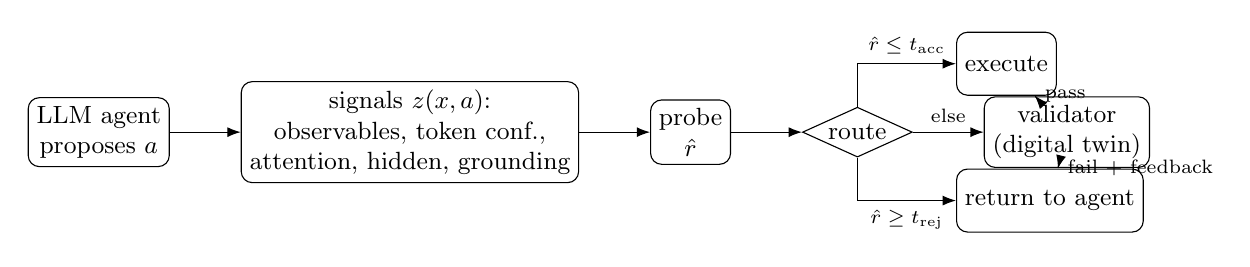
\begin{tikzpicture}[node distance=7mm and 9mm, every node/.style={font=\small},
  box/.style={draw, rounded corners, align=center, minimum height=8mm, inner sep=3pt},
  dec/.style={draw, diamond, aspect=2.2, align=center, inner sep=1pt}]
\node[box] (agent) {LLM agent\\proposes $a$};
\node[box, right=of agent] (sig) {signals $z(x,a)$:\\observables, token conf.,\\attention, hidden, grounding};
\node[box, right=of sig] (probe) {probe\\$\hat r$};
\node[dec, right=of probe] (route) {route};
\node[box, above right=3mm and 9mm of route] (exec) {execute};
\node[box, right=9mm of route] (val) {validator\\(digital twin)};
\node[box, below right=3mm and 9mm of route] (rej) {return to agent};
\draw[-{Latex}] (agent) -- (sig);
\draw[-{Latex}] (sig) -- (probe);
\draw[-{Latex}] (probe) -- (route);
\draw[-{Latex}] (route) |- node[pos=0.75, above]{\scriptsize $\hat r\le t_{\mathrm{acc}}$} (exec);
\draw[-{Latex}] (route) -- node[above]{\scriptsize else} (val);
\draw[-{Latex}] (route) |- node[pos=0.75, below]{\scriptsize $\hat r\ge t_{\mathrm{rej}}$} (rej);
\draw[-{Latex}] (val) -- node[right]{\scriptsize pass} (exec);
\draw[-{Latex}] (val) -- node[right]{\scriptsize fail + feedback} (rej);
\end{tikzpicture}
\caption{Skip-the-validator routing. A probe estimates the failure risk of each proposal from the chosen signals;
confident proposals are executed and clearly failing ones returned to the agent without a validator call. Under the
first-proposal-only rule (R0), retries are never accepted unchecked.}
\label{fig:routing}
\end{figure}

\subsection{Signals}
All internal signals are read from the forward pass that produces the proposal, at four relative depths of the
network (0.25, 0.5, 0.75 and 1.0).
\begin{itemize}
\item \textbf{Observables.} Task-state features visible in the prompt and features of the proposed action. In path
planning: graph size, query and path properties. In the CSTR: the measured temperature, level and actuator commands,
alarm flags, and the proposed setpoint changes. A \emph{plant-readings-only} variant omits the action features.
\item \textbf{Token confidence.} Log-probability, entropy and top-two margin statistics of the answer tokens, overall
and for numeric tokens.
\item \textbf{Attention by prompt region.} The share of attention mass from answer tokens to each prompt region
(instructions, knowledge graph or graph description, task state), with head-mean and head-max aggregation and
attention entropy.
\item \textbf{Hidden states.} The residual-stream vector at the last prompt token and its mean over answer tokens,
standardised and reduced to 64 principal components fitted on training data.
\item \textbf{Region-based attention grounding.} For each decision-relevant answer token, the share of attention on
the prompt region that decides it, relative to all task-content regions. In path planning, a step $u\to v$ is legal
only if $v$ appears in the adjacency line of $u$; the deciding region for the tokens of $v$ is that line. In the CSTR,
the deciding regions for each setpoint are the plant measurements that indicate its effect and the knowledge-graph
statements of the controller and balance equations that link it to the plant (pre-registered before computation).
Features are summarised over steps or setpoints (minimum, mean) and layers.
\end{itemize}
Combinations (\emph{all internals} = token confidence + attention + hidden states; \emph{observables + internals};
\emph{observables + grounding}) are fitted as single probes.

\subsection{Probes and thresholds}
Each signal set is fitted with an $\ell_2$-regularised logistic regression on the training partition (median
imputation and standardisation fitted on training data) and Platt-calibrated on a calibration partition. Thresholds
are chosen on the pooled development partitions $\mathcal D$ for a tolerance $X$ on the failure rate among unchecked
accepts. The accept threshold is the largest $t$ for which a one-sided Clopper--Pearson upper bound
\citep{clopper1934} at level $1-\delta_{\mathrm{sel}}$ ($\delta_{\mathrm{sel}}=0.05$) on the failure rate of
$\{a\in\mathcal D:\hat r(a)\le t\}$ is at most $X$. This bound-based rule replaced an initial point-estimate rule,
which proved too loose on certification data; the change was pre-registered before any affected test data were
analysed. The reject threshold is the smallest $t$ for which at least 95\% of $\{a\in\mathcal D:\hat r(a)\ge t\}$
fail. We report $X=10\%$ as primary and $X=5\%$ as secondary.

\subsection{Certification}
On an independent certification set used once, a screen is \emph{certified} at $X$ if the one-sided Clopper--Pearson
upper bound on the failure rate among its unchecked accepts, at level $1-\delta/K$ with $\delta=0.05$ and $K$ the
number of signal sets compared (Bonferroni), is at most $X$. A bound below $X$ requires a sufficiently large accept
set: with $K=11$ and no failures, at least about 52 unchecked accepts are needed at $X=10\%$, which was stated in
advance as a power limit for the 500-episode CSTR certification sets.

\subsection{Closed-loop evaluation and cost}
In closed loop each episode runs the propose--route--(validate)--retry loop with a budget of six proposals; if no
proposal is executed, the current setpoints are held. The executed outcome is the digital twin's verdict on the
executed setpoints with the plant's own future disturbances. We compare the screens with always-validate,
never-validate, and random routing at the combined probe's development accept and reject rates. Under the
\emph{first-proposal-only rule} (R0), a retry that the probe would accept is validated instead. The compute per
episode is
\begin{equation}
C = \sum_{\text{proposals}} \left(c_{\mathrm{gen}} + c_{\mathrm{feat}}\right) + n_{\mathrm{val}}\,c_{\mathrm{val}},
\end{equation}
where $c_{\mathrm{gen}}$ is generation time, $c_{\mathrm{feat}}$ the extra feature passes (zero for observables),
$n_{\mathrm{val}}$ the number of validator calls and $c_{\mathrm{val}}$ the validator cost per call. The screen's cost
does not depend on the simulator, whereas $c_{\mathrm{val}}$ grows with simulation horizon and fidelity. Because the
plant is paused during decisions, the logged decisions do not depend on $c_{\mathrm{val}}$, so $C$ can be recomputed
exactly for any validator cost, and the break-even cost $c^{*}_{\mathrm{val}}$ at which a screen matches
always-validate follows directly.

\section{Experimental setup}\label{sec:setup}

\subsection{Domain 1: graph path planning (exact validator)}
Each instance is a directed graph with 5, 10, 15 or 20 nodes, given in the prompt as one adjacency line per node,
together with a start and a goal node and one worked example. The agent returns the path as a JSON list. The
validator checks that the path starts and ends correctly and that every step $u\to v$ is an edge, i.e.\ that $v$
appears in the adjacency line of $u$. This validator is exact and costs microseconds, so this domain measures the
quality of the screens; compute savings are only meaningful in the second domain. Graphs are disjoint across all
datasets. Probes are fitted on a development set of 3000 graphs (1500 training, 500 calibration, 500 threshold
selection, 500 test) and evaluated once on a fresh certification set of 3000 graphs that had not been used before
(Table~\ref{tab:datasets}).

\subsection{Domain 2: CSTR fault recovery (digital-twin validator)}
The plant is the CSTR case study of \citep{car_todo}: a jacketed reactor with level, temperature and inlet-flow PID
loops, a monitoring layer that triggers the agent when the process leaves its safe operating region, and a digital
twin. Each episode draws a nominal plant (heat-transfer coefficient, feed and coolant temperatures, inlet
concentrations, coolant capacity, nominal level and feed setpoints), a fault family (jacket fouling, outlet pump
degradation, cooling valve stuck partly closed, outlet blockage), a continuous fault severity and an onset time
(1500--5000\,s). The plant is simulated to the first monitor trigger, and the snapshot at that moment is the agent's
task. Episodes that never trigger, or trigger before the fault onset, are redrawn within the same fault family.

The prompt contains the agent's role, the plant's knowledge graph in Turtle (process operators, controllers and the
mass and energy balance equations), the snapshot (measurements, actuator commands, alarms and current setpoints),
the goal and the admissible setpoint ranges. The prompt is deliberately \emph{neutral}: it states plant physics and
the acceptance criteria but gives no advice on which setpoint to change, in which direction or by how much, so that
failures reflect the model's own reasoning rather than prompt wording. The agent returns three setpoints (temperature,
level, feed flow) as JSON after a short justification.

The validator simulates the plant forward from the snapshot under the proposed setpoints, with the plant's own future
disturbances, to the end of the horizon. A proposal passes if the plant reaches the safe state (temperature at most
313\,K, level within 2--11, no overflow, no actuator saturated while the temperature is away from 310\,K) within
600\,s, holds it for 60 consecutive seconds, and remains safe for at least 80\% of the remaining run. One validation
took 7.8--11.6\,s on our hardware, depending on concurrent load.

Fault severities were calibrated without the LLM so that the reference model's (Qwen2.5-3B) first proposals pass in
roughly 30\% of episodes, which gives enough passing proposals to train and certify an accept decision. This is a
property of the dataset, not a target for the agents; pass rates of the other models range from 17\% to 35\%. The
5000 episodes are partitioned by episode into training (3000), calibration (500), threshold selection (500), test
(500) and certification (500), each with equal numbers per fault family. A further 400 fresh episodes, disjoint from
all others, are used for the closed loop.

\subsection{Models and inference}
Qwen2.5-1.5B, Qwen2.5-3B and Qwen2.5-7B \citep{qwen2025}, Llama-3.2-3B \citep{llama3} and SmolLM2-1.7B
\citep{allal2025smollm2} instruction-tuned models were run locally in bfloat16, except Qwen2.5-7B, which was run with
4-bit NF4 weights \citep{dettmers2023qlora} to fit an 8\,GB laptop GPU (NVIDIA RTX 4060). Decoding is greedy, so every
proposal is reproducible. The knowledge graph was exported once and frozen, so all prompts are identical across runs.

\subsection{Pre-registration and data hygiene}
For each study we froze a pre-registration before computing the relevant features or outcomes, recording later
changes as dated amendments made before the affected data were examined: the change of primary endpoint to validator
calls skipped, the bound-based accept rule, additional signal combinations, the closed-loop policies, the
first-proposal-only rule and a pilot gate for SmolLM2 in the CSTR. Test and certification partitions were evaluated
once per model with frozen probes and thresholds. Two analyses are labelled exploratory: the CSTR results of
Qwen2.5-3B under the bound-based rule (its sealed sets had been used once under the earlier rule), and the CSTR
closed-loop probes of Qwen2.5-3B, which come from that exploratory freeze (the closed-loop episodes themselves are
fresh). Where a run failed for technical reasons (GPU memory exhaustion, a crashed simulator worker), it was resumed
from its saved records; no records were discarded.

\begin{table}[t]
\centering
\small
\caption{Evaluation sets used for the confirmatory results (one candidate per graph or episode). FSM: fresh certification set, never used before evaluation. CSTR: sealed test and certification partitions, each evaluated once.}
\label{tab:datasets}
\begin{tabular}{llrrr}
\toprule
Domain & Model & Set & Eligible & Failure rate \\
\midrule
FSM & Qwen-3B & cert2 (fresh) & 2992 & 0.51 \\
FSM & Llama-3B & cert2 (fresh) & 2995 & 0.63 \\
FSM & Qwen-1.5B & cert2 (fresh) & 2945 & 0.68 \\
FSM & SmolLM-1.7B & cert2 (fresh) & 2946 & 0.83 \\
FSM & Qwen-7B & cert2 (fresh) & 2973 & 0.49 \\
CSTR & Qwen-1.5B & test_iid & 494 & 0.67 \\
CSTR & Qwen-1.5B & cert & 492 & 0.66 \\
CSTR & Qwen-3B$^\dagger$ & test_iid & 493 & 0.71 \\
CSTR & Qwen-3B$^\dagger$ & cert & 498 & 0.67 \\
CSTR & Qwen-7B & test_iid & 499 & 0.79 \\
CSTR & Qwen-7B & cert & 498 & 0.80 \\
CSTR & Llama-3B & test_iid & 473 & 0.84 \\
CSTR & Llama-3B & cert & 474 & 0.83 \\
CSTR & SmolLM-1.7B & test_iid & 499 & 0.67 \\
CSTR & SmolLM-1.7B & cert & 496 & 0.66 \\
\bottomrule
\end{tabular}
\end{table}


\section{Offline results: how many validator calls can each signal skip?}\label{sec:results}

\subsection{Path planning}
Table~\ref{tab:skip-fsm} reports the share of validator calls skipped on the fresh certification set. Observable
features alone skip 16--85\% of calls depending on the model, with the failure bound among unchecked accepts
certified for three models. Adding internal signals increases the share of skipped calls for four of the five models
(Fig.~\ref{fig:delta}): by 14.0 points [12.4, 15.5] for Qwen2.5-3B, 15.0 [13.2, 16.9] for Llama-3.2-3B and 6.2 [4.8,
7.5] for SmolLM2 with the full combination, and by 5.1 points [3.7, 6.6] for Qwen2.5-1.5B with grounding alone. For
Llama-3.2-3B, region-based grounding alone carries the whole gain (+15.5 [13.8, 17.3]), and most of these screens
remain certified. Qwen2.5-7B is the exception: its observable screen (15.7\% skipped, certified) is not improved by
internal signals. Internal signals alone skip fewer calls than observables for every model, and token confidence is
the weakest signal throughout.

\begin{table*}[t]
\centering
\small
\caption{FSM: share of validator calls skipped (\%) per signal on the fresh certification set (tolerance $X=10\%$). Bold: failure rate among unchecked accepts certified $\le 10\%$ (one-sided Clopper--Pearson, Bonferroni over signals). $^{+}$/$^{-}$: significantly more/fewer calls skipped than observables (paired bootstrap 95\% CI).}
\label{tab:skip-fsm}
\begin{tabular}{lrrrrr}
\toprule
Signal & Qwen-1.5B & Qwen-3B & Qwen-7B & Llama-3B & SmolLM-1.7B \\
\midrule
Observables & \textbf{40} & \textbf{21} & \textbf{16} & 43 & 85 \\
\midrule
Obs. + grounding & \textbf{46}$^{+}$ & \textbf{21} & 22$^{+}$ & \textbf{59}$^{+}$ & 85 \\
Obs. + all internals & \textbf{37}$^{-}$ & \textbf{32}$^{+}$ & 15 & \textbf{47}$^{+}$ & 79$^{-}$ \\
Obs. + internals + grounding & \textbf{40} & \textbf{34}$^{+}$ & \textbf{15} & \textbf{58}$^{+}$ & 91$^{+}$ \\
\midrule
Region grounding & \textbf{31}$^{-}$ & \textbf{14}$^{-}$ & \textbf{3}$^{-}$ & \textbf{31}$^{-}$ & 80$^{-}$ \\
Attention (regions) & \textbf{35}$^{-}$ & \textbf{21} & 13$^{-}$ & 17$^{-}$ & 75$^{-}$ \\
Hidden states & 22$^{-}$ & \textbf{24}$^{+}$ & 10$^{-}$ & 27$^{-}$ & 74$^{-}$ \\
All internals & \textbf{25}$^{-}$ & \textbf{25}$^{+}$ & \textbf{9}$^{-}$ & \textbf{31}$^{-}$ & 76$^{-}$ \\
All internals + grounding & \textbf{38}$^{-}$ & \textbf{23}$^{+}$ & \textbf{11}$^{-}$ & \textbf{36}$^{-}$ & 79$^{-}$ \\
Token confidence & 13$^{-}$ & 18$^{-}$ & 0$^{-}$ & 14$^{-}$ & 56$^{-}$ \\
\bottomrule
\end{tabular}
\end{table*}


\subsection{CSTR fault recovery}
In the CSTR (Table~\ref{tab:skip-cstr}), observables skip 41--86\% of calls. The picture for internal signals is
different from path planning. They add significantly for three of five models, each in a different way. For
SmolLM2, both the full combination (+4.8 [1.4, 8.3]) and grounding alone (+3.8 [1.4, 6.2]) skip more calls. For
Llama-3.2-3B, adding internals does not change the share skipped but halves the good proposals rejected unchecked
(16 to 8 of 79, difference $-8$ [$-15$, $-2$]). For Qwen2.5-3B, internals make unchecked accepts possible at all under
the bound-based rule (exploratory). For Qwen2.5-1.5B and Qwen2.5-7B, observables are as good as or better than any
combination. Internals alone skip 10--53\% of calls, almost entirely by rejecting clearly failing proposals; the
all-internals screen executes at most one failing proposal unchecked for any model, although single internal signals
can be less safe (hidden states alone for SmolLM2: 9 failing of 65 accepted).

No CSTR screen is certified at $X=10\%$. This is the power limit stated in advance: with 500 certification episodes
and accept sets of 35--130 proposals, the Bonferroni-corrected bound cannot fall below 10\% even with few failures.
The observed failure rates among unchecked accepts were 4--12\% for the observable screens that accepted any
proposal.

\begin{table*}[t]
\centering
\small
\caption{CSTR: share of validator calls skipped (\%) per signal on the certification partition ($X=10\%$); notation as in Table~\ref{tab:skip-fsm}. $^\dagger$Qwen-3B: exploratory re-analysis under the bound-based rule (its sealed sets had been used once before the rule change).}
\label{tab:skip-cstr}
\begin{tabular}{lrrrrr}
\toprule
Signal & Qwen-1.5B & Qwen-3B$^\dagger$ & Qwen-7B & Llama-3B & SmolLM-1.7B \\
\midrule
Observables & 63 & 41 & 86 & 71 & 61 \\
\midrule
Obs. + grounding & 60$^{-}$ & 39 & 86 & 75$^{+}$ & 65$^{+}$ \\
Obs. + all internals & 61 & 51 & 83 & 72 & 66$^{+}$ \\
Obs. + internals + grounding & 61 & 50 & 80$^{-}$ & 74 & 66$^{+}$ \\
\midrule
Region grounding & 27$^{-}$ & 10 & 47$^{-}$ & 38$^{-}$ & 24$^{-}$ \\
Attention (regions) & 30$^{-}$ & 15 & 49$^{-}$ & 48$^{-}$ & 31$^{-}$ \\
Hidden states & 29$^{-}$ & 13 & 50$^{-}$ & 48$^{-}$ & 45$^{-}$ \\
All internals & 29$^{-}$ & 15 & 47$^{-}$ & 53$^{-}$ & 40$^{-}$ \\
All internals + grounding & 28$^{-}$ & 12 & 48$^{-}$ & 53$^{-}$ & 41$^{-}$ \\
Token confidence & 4$^{-}$ & 0 & 17$^{-}$ & 34$^{-}$ & 22$^{-}$ \\
\bottomrule
\end{tabular}
\end{table*}


\begin{figure}[t]
\centering
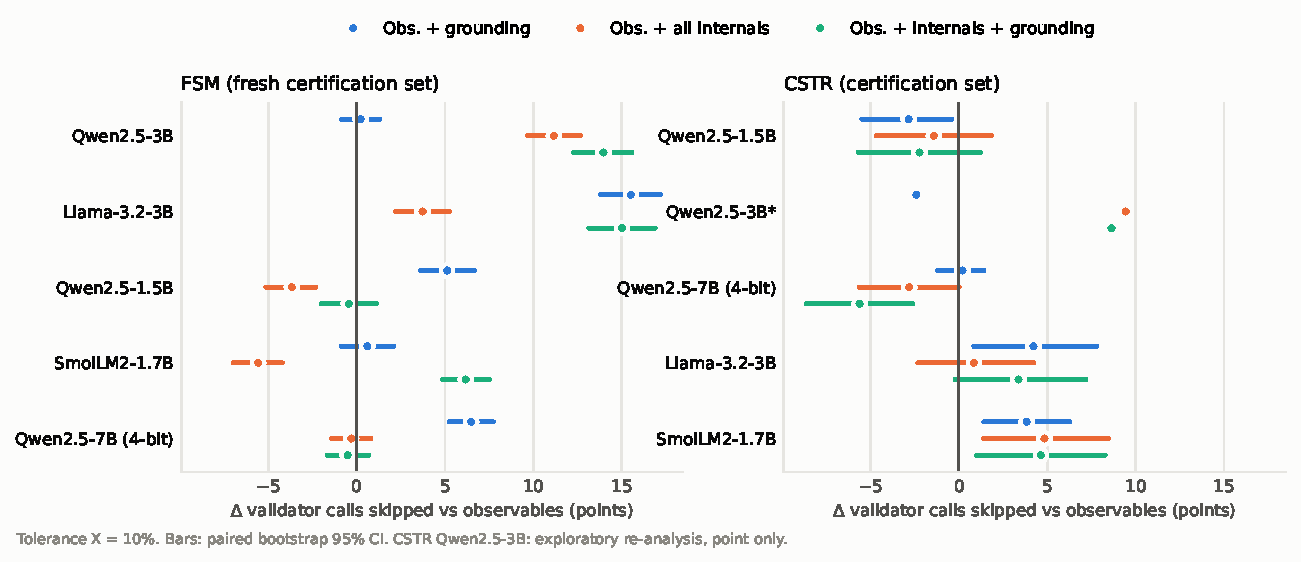
\includegraphics[width=\textwidth]{figures/delta_vs_observables.pdf}
\caption{Change in validator calls skipped relative to the observable screen when grounding, all internal signals,
or both are added (tolerance $X=10\%$, paired bootstrap 95\% CI). Left: path planning, fresh certification set.
Right: CSTR, certification partition.}
\label{fig:delta}
\end{figure}

\subsection{Why internals help in one domain and not the other}
Table~\ref{tab:mechanism} tests the mechanism behind region-based grounding directly: does low attention on the
deciding prompt region predict a failing answer? In path planning it does, strongly, for all five models (AUROC
0.75--0.88). At the level of individual steps, an illegal step receives markedly less attention on the source node's
adjacency line than a legal one (AUROC 0.64--0.81 for the four models analysed at step level). Path-planning failures
are retrieval failures: the information that decides the step is in the prompt, and the model did not consult it.

In the CSTR the signal is weak or absent for three models (0.48--0.52) and moderate for the two smallest (0.66 for
SmolLM2, 0.72 for Qwen2.5-1.5B). A pre-registered test for Qwen2.5-3B makes the contrast explicit. Proposals that
raise the feed while the cooling is saturated and the reactor is hot, a move the physics in the prompt rules out,
receive slightly \emph{more} attention on the physics section than other proposals (AUROC 0.31 for the predicted
direction). The model reads the relevant physics and still reasons to the wrong action. Attention grounding detects
the first kind of failure, not the second, which is why its value is domain dependent. This is consistent with the
view that attention is useful as a predictive signal without being a full explanation of model behaviour
\citep{jain2019attention,wiegreffe2019attention}.

\begin{table}[t]
\centering
\small
\caption{Does low attention on the prompt region that decides the answer predict failure? AUROC of the negative minimum grounding share for answer failure (train + development data; 0.5 = no signal).}
\label{tab:mechanism}
\begin{tabular}{lrr}
\toprule
Model & FSM & CSTR \\
\midrule
Qwen-1.5B & 0.84 & 0.72 \\
Qwen-3B & 0.75 & 0.50 \\
Qwen-7B & 0.72 & 0.48 \\
Llama-3B & 0.84 & 0.52 \\
SmolLM-1.7B & 0.88 & 0.66 \\
\bottomrule
\end{tabular}
\end{table}


\subsection{Robustness to plant and fault shift}
A screen is only useful if it remains valid when the plant population changes. In a pre-registered shift analysis
(Table~\ref{tab:shift}) we fitted probes on one part of the plant and fault space and evaluated them on another,
without recalibration: low to high nominal feed rate (visible in the prompt), low to high heat-transfer coefficient
(not visible), and each fault family held out in turn. All signals degrade under the feed and fault-family shifts, by
0.04--0.28 AUROC for the observable screen, whereas the cooling shift is nearly harmless. Contrary to our
pre-registered expectation, internal signals did not degrade less than observables, and adding them made unchecked
accepts \emph{less} safe on unseen fault types for one model. An earlier, larger shift (one training plant to a varied
population, under a different prompt) had favoured internal signals; we report both and conclude that the screens
must be recalibrated when the plant or fault population changes.

\begin{table}[t]
\centering
\small
\caption{AUROC for failure on the target part of each pre-registered shift (probes fitted on the source part only). Control: random split of the same size.}
\label{tab:shift}
\begin{tabular}{llrrrr}
\toprule
Model & Signal & Control & Feed & Cooling & Fault family \\
\midrule
Qwen-1.5B & Observables & 0.93 & 0.70 & 0.91 & 0.72 \\
 & Obs. + all internals & 0.92 & 0.72 & 0.90 & 0.74 \\
 & All internals & 0.80 & 0.64 & 0.79 & 0.66 \\
 & Token confidence & 0.65 & 0.54 & 0.63 & 0.50 \\
\midrule
Qwen-3B & Observables & 0.87 & 0.73 & 0.86 & 0.80 \\
 & Obs. + all internals & 0.85 & 0.74 & 0.85 & 0.74 \\
 & All internals & 0.71 & 0.60 & 0.72 & 0.62 \\
 & Token confidence & 0.57 & 0.48 & 0.55 & 0.50 \\
\midrule
Qwen-7B & Observables & 0.93 & 0.66 & 0.92 & 0.77 \\
 & Obs. + all internals & 0.92 & 0.65 & 0.91 & 0.71 \\
 & All internals & 0.80 & 0.52 & 0.77 & 0.55 \\
 & Token confidence & 0.68 & 0.47 & 0.66 & 0.54 \\
\midrule
Llama-3B & Observables & 0.90 & 0.86 & 0.91 & 0.80 \\
 & Obs. + all internals & 0.92 & 0.91 & 0.93 & 0.82 \\
 & All internals & 0.84 & 0.83 & 0.86 & 0.71 \\
 & Token confidence & 0.63 & 0.57 & 0.66 & 0.57 \\
\bottomrule
\end{tabular}
\end{table}


\section{Closed-loop results and compute}\label{sec:closedloop}

\subsection{Safety and recovery}
Table~\ref{tab:closedloop} reports 400 fresh CSTR episodes per model, with every policy run on the same episodes.
Validating every proposal recovers 34--54\% of episodes. Never validating executes a failing action in 64--80\% of
episodes, and random routing at the screens' skip rates executes 107--186 failing actions (except for Llama-3.2-3B,
whose random policy, like its probes, never accepted). The trained screens execute far fewer failing actions while
avoiding 29--90\% of validator calls. On first proposals they behave as they did offline: the observable screen
executed 0--13 failing actions unchecked per 400 episodes.

\paragraph{Retries are a distribution shift for internal signals} For two models, probes that use internal signals
accepted many failing \emph{retries}: the combined probe of Qwen2.5-7B executed 165 failing actions, 161 of them on
retries, and SmolLM2's combined and internals-only probes executed 237 and 243, nearly all on retries. The probes were
trained on first proposals. A retry prompt contains the validator's failure feedback, which shifts the model's
internal state, and the probes misread failing retries as safe. Observable-only probes, whose inputs do not change
between first proposals and retries, were unaffected.

\paragraph{The first-proposal-only rule} Allowing unchecked execution only for first proposals (R0) and validating
every retry removes these failures (Table~\ref{tab:closedloop}). For SmolLM2, failing executions fell from 237 to 11
(combined) and from 243 to 2 (internals only), with recovery unchanged ($-1.0$ [$-2.0$, $-0.3$] and $-0.5$ [$-1.3$,
0.0] points relative to always-validate) and validator calls still reduced by 65\% and 42\%. For Qwen2.5-7B the
combined probe's failing executions fell from 165 to 4, with recovery unchanged within uncertainty
($-1.5$ [$-4.5$, $+1.5$] points) and validator calls still reduced by 41\%. For the other three
models the rule changes nothing, because their probes accepted no failing retries. With R0, an internals-only screen,
which uses no plant measurements and no model of the plant, avoided 29--65\% of validator calls across the five models
while executing 0--2 failing actions unchecked.

\paragraph{Where recovery is lost} The screens' recovery cost ranges from $-0.5$ to $-18.5$ points. It comes from
unchecked \emph{rejects}, not from unsafe accepts: each reject requires a new proposal and consumes the six-proposal
budget, and some rejected proposals were good (up to 0.45 per episode for Qwen2.5-3B's internals-only screen). For
Llama-3.2-3B, whose proposals rarely pass, every skipped call is a reject, and recovery falls by 4.0 (internals only)
to 18.5 (observables) points. For the two smallest models, validation itself does not improve recovery
(never-validate recovers as often as always-validate) because they mostly repeat their proposals; there, validation
and the screens serve to prevent the execution of failing actions.

\begin{table*}[t]
\centering
\small
\caption{Closed-loop CSTR recovery on 400 fresh episodes per model. $\Delta$: paired difference to always-validate (percentage points, bootstrap 95\% CI over episodes). Unsafe: failing actions executed without validation. Calls: validator calls avoided relative to always-validate. R0: the probe may skip validation only for first proposals (retries are always validated).}
\label{tab:closedloop}
\begin{tabular}{llrrrr}
\toprule
Model & Policy & Recovered (\%) & $\Delta$ recovered & Unsafe & Calls avoided \\
\midrule
Qwen-1.5B & Always validate & 34.5 & -- & 0 & -- \\
 & Observables & 33.0 & -1.5 [-3.0, -0.2] & 12 & 67\% \\
 & Obs.+int.+grd. & 33.2 & -1.2 [-2.5, +0.0] & 9 & 64\% \\
 & Internals only & 33.2 & -1.2 [-2.5, -0.2] & 0 & 35\% \\
 & Random (matched) & 33.8 & -0.8 [-1.8, +0.0] & 186 & 60\% \\
 & Never validate & 34.5 & +0.0 [+0.0, +0.0] & 259 & 100\% \\
\midrule
Qwen-3B & Always validate & 43.8 & -- & 0 & -- \\
 & Observables & 41.0 & -2.8 [-5.8, +0.2] & 0 & 47\% \\
 & Obs.+int.+grd. & 37.0 & -6.8 [-10.2, -3.5] & 1 & 72\% \\
 & Internals only & 30.0 & -13.8 [-17.5, -10.5] & 0 & 65\% \\
 & Random (matched) & 37.8 & -6.0 [-9.0, -3.0] & 110 & 47\% \\
 & Never validate & 30.0 & -13.8 [-17.2, -10.5] & 274 & 100\% \\
\midrule
Qwen-7B & Always validate & 0.0 & -- & 0 & -- \\
 & Observables & 0.0 & +0.0 [+0.0, +0.0] & 1 & 60\% \\
 & Observables, R0 & 0.0 & +0.0 [+0.0, +0.0] & 0 & 20\% \\
 & Obs.+int.+grd. & 0.0 & +0.0 [+0.0, +0.0] & 1 & 80\% \\
 & Obs.+int.+grd., R0 & 0.0 & +0.0 [+0.0, +0.0] & 0 & 20\% \\
 & Internals only & 0.0 & +0.0 [+0.0, +0.0] & 0 & 20\% \\
 & Internals only, R0 & 0.0 & +0.0 [+0.0, +0.0] & 0 & 20\% \\
 & Random (matched) & 0.0 & +0.0 [+0.0, +0.0] & 1 & 40\% \\
 & Never validate & 0.0 & +0.0 [+0.0, +0.0] & 2 & 100\% \\
\midrule
Llama-3B & Always validate & 53.8 & -- & 0 & -- \\
 & Observables & 35.2 & -18.5 [-23.5, -13.2] & 0 & 62\% \\
 & Obs.+int.+grd. & 44.5 & -9.2 [-13.8, -4.5] & 0 & 45\% \\
 & Internals only & 49.8 & -4.0 [-8.0, +0.0] & 0 & 29\% \\
 & Random (matched) & 29.5 & -24.2 [-29.2, -19.0] & 0 & 68\% \\
 & Never validate & 15.2 & -38.5 [-43.2, -33.8] & 312 & 100\% \\
\midrule
SmolLM-1.7B & Always validate & 36.5 & -- & 0 & -- \\
 & Observables & 35.2 & -1.2 [-2.5, -0.2] & 13 & 62\% \\
 & Observables, R0 & 35.2 & -1.2 [-2.5, -0.2] & 13 & 62\% \\
 & Obs.+int.+grd. & 35.0 & -1.5 [-2.8, -0.5] & 237 & 66\% \\
 & Obs.+int.+grd., R0 & 35.5 & -1.0 [-2.0, -0.2] & 11 & 65\% \\
 & Internals only & 35.5 & -1.0 [-2.0, -0.2] & 243 & 44\% \\
 & Internals only, R0 & 36.0 & -0.5 [-1.2, +0.0] & 2 & 42\% \\
 & Random (matched) & 34.0 & -2.5 [-4.2, -1.0] & 172 & 65\% \\
 & Never validate & 36.0 & -0.5 [-1.2, +0.0] & 254 & 100\% \\
\bottomrule
\end{tabular}
\end{table*}


\subsection{Compute}
Generation dominates the per-episode compute on our hardware (Table~\ref{tab:costs}); the feature passes needed by
internal signals add 2--14\,s per episode (the most for Llama-3.2-3B). At the measured validator cost (7.8--11.6\,s per call), the screens save
little or cost time, because every unchecked reject triggers a regeneration that costs about as much as the
validation it replaces. The screen's cost, however, is independent of the simulator, while the validator's cost grows
with the simulated horizon, model fidelity and number of scenarios. Re-costing the same decisions
(Fig.~\ref{fig:costs}) shows savings of 11--49\% of total compute at 30\,s per validation and
21--64\% at 60\,s for four of the five models, with break-even validator costs of 2--18\,s. Llama-3.2-3B is
the exception: since it is screened only by rejection, its break-even lies above 70\,s, and its timings are
additionally inflated by GPU memory pressure in our runs.

\begin{table*}[t]
\centering
\small
\caption{Compute per episode relative to always-validate (positive = saving). The logged closed-loop decisions do not depend on validator latency (the plant is paused during decisions), so the same decisions are re-costed exactly for a validator taking 30\,s or 60\,s per call. Break-even: validator cost per call above which the policy saves time.}
\label{tab:costs}
\begin{tabular}{llrrrr}
\toprule
Model & Policy & Measured & 30\,s & 60\,s & Break-even (s) \\
\midrule
Qwen-1.5B & Observables probe & +11\% & +28\% & +40\% & 3 \\
 & Obs. + internals + grounding probe & +5\% & +23\% & +36\% & 7 \\
 & Internals-only probe & +6\% & +14\% & +21\% & 3 \\
\midrule
Qwen-3B & Observables probe & +2\% & +21\% & +30\% & 7 \\
 & Obs. + internals + grounding probe & -4\% & +28\% & +44\% & 10 \\
 & Internals-only probe & -19\% & +16\% & +34\% & 17 \\
\midrule
Llama-3B & Observables probe & -40\% & -22\% & -5\% & 73 \\
 & Obs. + internals + grounding probe & -40\% & -24\% & -11\% & 97 \\
 & Internals-only probe & -29\% & -18\% & -9\% & 107 \\
\midrule
Qwen-7B & Observables probe & +18\% & +49\% & +64\% & 2 \\
 & Observables probe, first-proposal-only & +17\% & +47\% & +62\% & 3 \\
 & Obs. + internals + grounding probe & +31\% & +50\% & +59\% & any \\
 & Obs. + internals + grounding, first-proposal-only & -1\% & +17\% & +26\% & 9 \\
 & Internals-only probe & -1\% & +18\% & +28\% & 9 \\
 & Internals-only, first-proposal-only & -2\% & +17\% & +27\% & 10 \\
\midrule
SmolLM-1.7B & Observables probe & +0\% & +24\% & +39\% & 12 \\
 & Observables probe, first-proposal-only & -7\% & +20\% & +36\% & 15 \\
 & Obs. + internals + grounding probe & +44\% & +52\% & +58\% & any \\
 & Obs. + internals + grounding, first-proposal-only & -1\% & +25\% & +41\% & 12 \\
 & Internals-only probe & +40\% & +42\% & +43\% & any \\
 & Internals-only, first-proposal-only & -9\% & +11\% & +23\% & 18 \\
\bottomrule
\end{tabular}
\end{table*}


\begin{figure}[t]
\centering
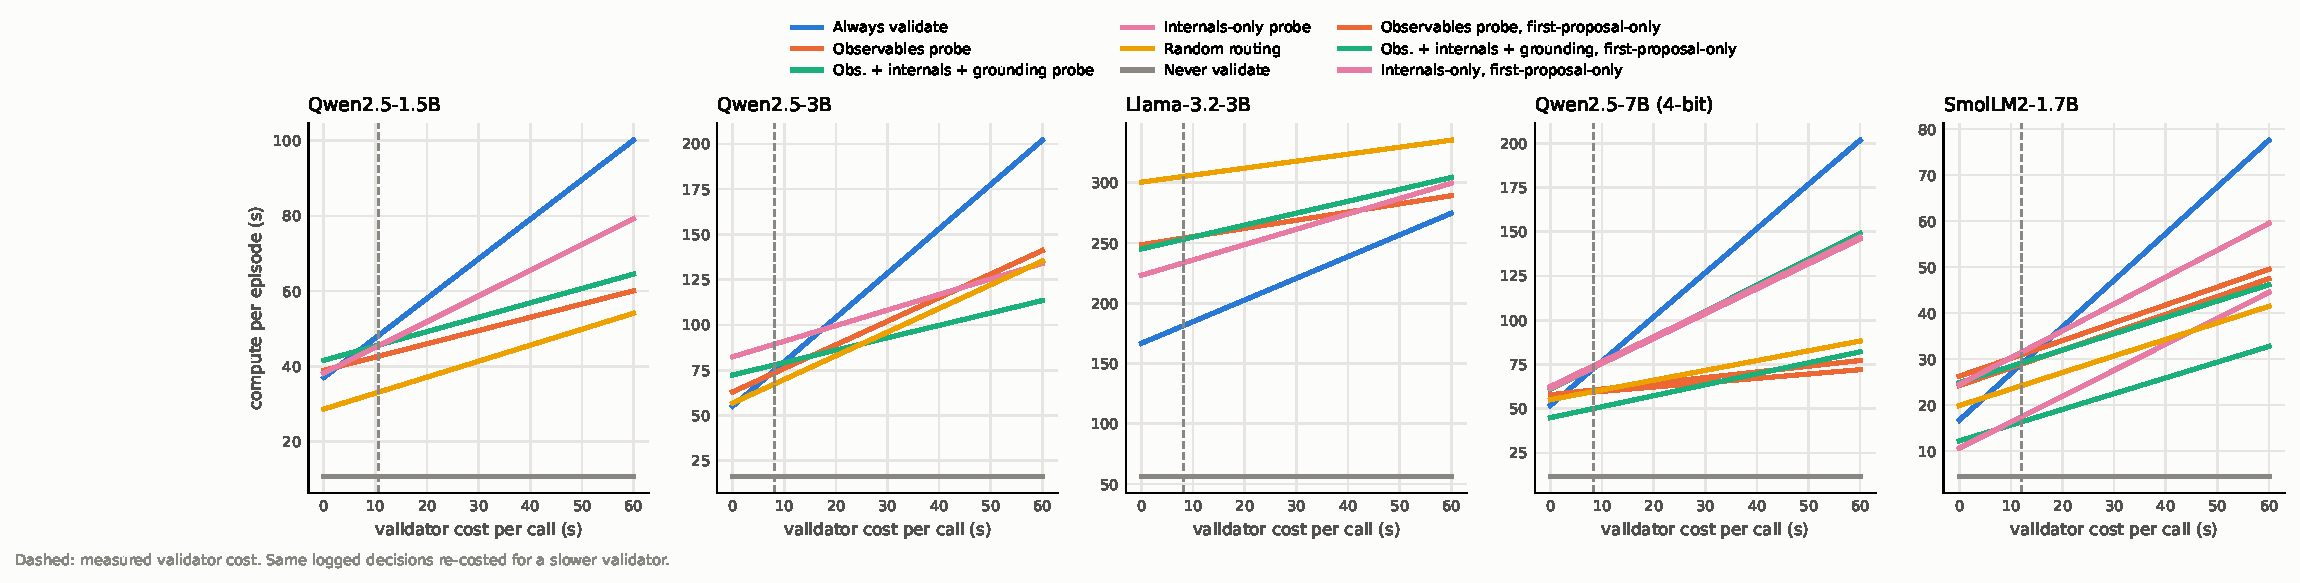
\includegraphics[width=\textwidth]{figures/closed_loop_compute_all.pdf}
\caption{Compute per closed-loop episode as a function of the validator's cost per call, for each model and policy.
The logged decisions are re-costed exactly; the dashed line marks the measured validator cost. Screens that avoid
validator calls overtake always-validate once validation costs more than a few seconds per call.}
\label{fig:costs}
\end{figure}

\section{Discussion}\label{sec:discussion}

\paragraph{When do model internals help an agent skip its validator?} Across two domains and five models, internal
signals were most useful when the agent's failures were failures to consult information that is in the prompt. In path
planning, a wrong step is almost always a step whose adjacency line the model did not attend to, and both
region-based grounding and the broader internal signals added 5--15 points of skipped validator calls on top of strong
observable baselines. In CSTR fault recovery, the relevant measurements and physics are short and salient; the model
attends to them and errs in the direction or size of its correction. There, the observable state and the proposed
action carry most of the information, and internal signals added little except for the smallest model. For
practitioners, the lesson is to diagnose the agent's failure mode before investing in internal-signal screens:
attention-based grounding pays off for retrieval-heavy tasks with long, structured contexts.

\paragraph{A practical recipe} Three design choices mattered more than the choice of signal. First, accept
thresholds must be chosen with a confidence bound, not a point estimate, or the realised failure rate among unchecked
accepts exceeds the tolerance on new data. Second, a screen trained on first proposals must not be applied to
retries without validation: retry prompts contain failure feedback, which shifts internal signals, and two of five
models' internal probes accepted failing retries; the first-proposal-only rule removed this at no measurable cost in
recovery. Third, the time saved depends on what a skipped call is replaced with. An unchecked accept saves a full
validation, but an unchecked reject triggers a regeneration, so screens save time only when validation is more
expensive than generation. This is exactly the regime that motivates selective validation: high-fidelity or
long-horizon simulators, scenario sets, or multi-unit plants, where validation cost grows while the agent's cost
stays fixed.

\paragraph{Plant models versus model internals} A natural objection is that a screen on plant measurements and
proposed setpoints is a learned surrogate of the plant rather than a statement about the agent. The plant-readings-only
baseline addresses this directly: for three models it skips nearly as many calls as the full observable screen
(the outcome is largely determined by the fault state), whereas for Qwen2.5-3B and Llama-3.2-3B it skips almost
none. More importantly, the internals-only screen uses no plant information at all, yet with the first-proposal-only
rule it avoided 29--65\% of validator calls while executing at most two failing actions unchecked in
2000 closed-loop episodes. The agent's own internal state therefore carries reliable information about when
its proposal can be rejected without simulation, independent of any plant model, even though it rarely suffices to
accept proposals unchecked.

\paragraph{Limitations} The study uses small and medium open-weight models (1.5--7B parameters), one of them
quantised, on a single laptop GPU; larger models may fail differently. The CSTR is one simulated plant with four
fault families, one prompt, and a paused plant during decisions; we make no claim about decision latency under real
time pressure. The validator doubles as the plant simulator in closed loop. The CSTR certification sets were too small
to certify accepts at a 10\% tolerance, as anticipated; larger certification sets are the remedy. The Qwen2.5-3B CSTR
screens come from an exploratory freeze. The probes were trained on first proposals only; training on retries is a
natural extension. Compute figures are specific to our hardware, but the re-costing makes the dependence on
validator cost explicit and transferable.

\section{Conclusion}\label{sec:conclusion}

LLM agents for process operations need not pay for a full simulation of every proposal. Learned risk screens that
combine the observable task state and proposed action with, where informative, the agent's internal signals skipped
16--91\% of validator calls in two domains with five models, with certified failure bounds where the data allowed and
far fewer unsafe executions than random skipping in closed loop. Internal signals, and region-based attention grounding
in particular, help when the agent's failures are failures to retrieve the information that decides its answer, and
help little when the agent retrieves the right information and reasons incorrectly. Two rules make such screens safe
and worthwhile in practice: accept proposals unchecked only on first proposals, with thresholds set by a confidence
bound; and deploy screening where validation is costly, since the screen's cost is fixed while the simulator's grows
with fidelity and horizon. Future work should train screens on retries, certify them on larger sets, and test them
with larger models, real-time constraints and plants with richer fault libraries.


\section*{CRediT authorship contribution statement}
\todo{CRediT roles per author.}

\section*{Declaration of competing interest}
The authors declare that they have no known competing financial interests or personal relationships that could have
appeared to influence the work reported in this paper.

\section*{Declaration of generative AI and AI-assisted technologies in the manuscript preparation process}
\todo{Elsevier requires this statement. Describe the use of AI assistance for code, analysis and drafting, and
confirm that the authors reviewed and edited the content and take full responsibility for it.}

\section*{Data availability}
Code, pre-registrations with dated amendments, frozen probes' manifests and all results tables are available at
\todo{repository URL / Zenodo DOI}. Raw model records and hidden-state arrays are available on request
\todo{or deposit on Zenodo}.

\section*{Acknowledgements}
\todo{Funding and acknowledgements.}

\bibliographystyle{elsarticle-num}
\bibliography{refs}

\end{document}
